\documentclass[fontsize=9pt,twocolumns,enabledeprecatedfontcommands]{scrartcl}
\usepackage[a4paper,textwidth=0.85\paperwidth,textheight=0.80\paperheight]{geometry}
%\usepackage[a4paper]{geometry}
\setlength{\columnsep}{0.03\paperwidth}

\usepackage[utf8]{inputenc}
\usepackage[english]{babel}
\usepackage[T1]{fontenc}
\usepackage{amsmath}
\usepackage{amsfonts}
\usepackage{amssymb}
\usepackage{epigraph}
\usepackage{paralist}
\usepackage{mathtools}%for smash operator

\usepackage{indentfirst} %adds indentation after sectioning

\usepackage{graphicx}
\usepackage{amsthm}
\usepackage{stmaryrd}  %pour Mapsto

\usepackage[bf,format=plain]{caption}
\usepackage{subcaption}
\usepackage{dblfloatfix}

\usepackage{url}
\usepackage{hyperref}
\usepackage{csquotes}

\usepackage[usenames,dvipsnames]{color}


\renewcommand\thesubfigure{\arabic{figure}} %subfigure have same counter as figures

\newcommand{\HRule}{\rule{0.9\linewidth}{0.05em}}

\addtokomafont{sectioning}{\rmfamily}
%\addtokomafont{part}{\huge}

\def\labelitemi{\textbf{--}}
\newenvironment{itemize'}
{ %\vspace{-0.75\topsep}
  \begin{itemize}
    \vspace{-\topsep}
    \setlength{\itemsep}{0pt}
    \setlength{\parskip}{0pt}
    \setlength{\parsep}{0pt}     }
{ \end{itemize} \vspace{-0.75\topsep}                 } 


\begin{document}
%\newgeometry{textheight=0.80\paperheight,textwidth=0.7\paperwidth}
%\begin{figure*}[h!]
\twocolumn[{
\noindent
\sffamily
\begin{center}
{\Large { Centre de Recherches Interdisciplinaires |  M1 AIV}}
%\\[1em]

\HRule

\vspace{1em}
{\Huge Solving optimization problems with search heuristics }\\[0.7em]

{\Huge Project report
}

\HRule
\\[2em]

\LARGE
\begin{tabular}{c}
	Arthur Carcano\\
\end{tabular}
\vspace{1em}
%\vfill
\end{center}}]


\newcommand{\wip}[1]{\textcolor{Purple}{WIPWIPWIPWIP #1 WIPWIPWIPWIP}}

\begin{abstract}
	We hereby present our solution to the traveling thief problem. Using a two phase algorithm inspired by \cite{Polyakovkiy}, we manage to reach solutions of about $16k$ on the \texttt{a280\_n279\_bounded-strongly-corr\_01.ttp} instance.
\end{abstract}

\section{Our algorithm}
Following the idea of Polyakovsiy \textit{et al.} \cite{Polyakovskiy} our algorithm runs in two phases. First a run for the travellign salesman problem is generated. Second, using this run, the algorithm plans which objects are to be picked up so as to maximize the total profit of our thief.

It noteworthy that, whereas our algorithm for the first phase is kind of intricate, the one used for the second phase is merely a classical simulated annealing.

\subsection{The TSP algorithm}
To solve the TSP problem, we first build a greedy solution which we then improve with different heuristics: basic node permutation, \textit{2-opt} and an permutation we call \textit{stitching} which is actually a specialization of \textit{3-opt}.

Both node inversion and stitching are accepting with a probability depending on a temperature $T$ that is exponentially decreasing.\\

We introduce the following notation, for any $x \in \mathcal{R}_+$ we define $\overline{x} = \max(1,x)$.

\subsection{Node inversion}:
This operation simply picks two nodes uniformly at random, compute $\Delta$ the difference of length of the tour if this two nodes are permuted and actually does this permutation with probability $\overline{e^{\frac{-\Delta}{T}}}$.

\subsection{Stitching}:
\begin{figure}
	
	\begin{subfigure}{0.5\textwidth}
		
		\centering
		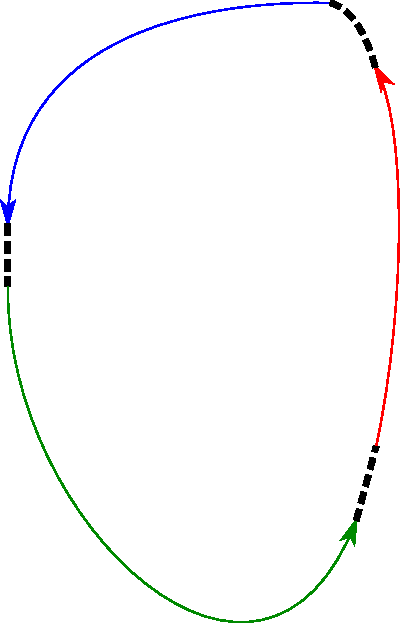
\includegraphics[angle=90,width=0.9\linewidth,height=0.15\textheight]{stitch1}
		\caption{Before stitching}
		\label{stitch1}
		
	\end{subfigure}
	\vspace{2em}
	\begin{subfigure}{0.5\textwidth}
		
		\centering
		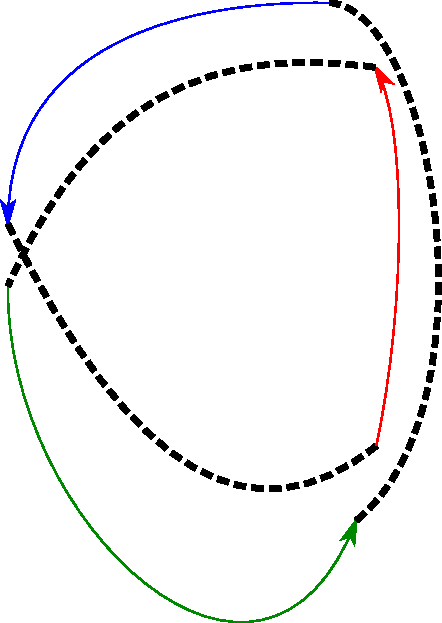
\includegraphics[angle=90,width=0.9\linewidth,height=0.15\textheight]{stitch2}
		\caption{After stitching}
		\label{stitch2}
		
	\end{subfigure}
	\captionsetup{format=plain}
	\caption{Illustration of the stitching operation}
	\label{stitch_fig}
	\centering
	%\vspace{0.25em}
	\rule{0.10\textwidth}{0.5pt}
	\vspace{-0.75em}
\end{figure}

As illustrated in figure \ref{stitch_fig}, the stitching of moving a part of the tour between two edges
\bibliographystyle{siam}
\bibliography{biblio}

\end{document}



%\begin{abstract}
